% !TeX spellcheck = es_ES
\documentclass[a4paper,11pt,twoside,openright]{book}

%%%%%%%%%%%%% Xeometría
\usepackage[a4paper,left=1.5cm,right=1cm, bottom=2.5cm,top=2.5cm]{geometry}

%%%%%%%%%%%%%%% Estilo
\usepackage[palette=starrynight]{nexus}

%%%%%%%%%%%%%%% Idioma
\usepackage[spanish]{babel}

%%%%%%%%%%%%%%% Fuentes tipográficas
\usepackage{amsmath}
\usepackage{kmath,kerkis}
\usepackage[T1]{fontenc}

%%%%%%%%%%%%%%%% hyperref
\usepackage[verbose]{hyperref}
\hypersetup{hidelinks}
\setlength{\XeTeXLinkMargin}{-1pt}


%%%%%%%%%%%%%%% Dos Columnas
\twocolumn
\setlength{\columnsep}{10mm}

%%%%%%%%%%%%%%% Gráficas
\usepackage{pgfplots}
\pgfplotsset
{	
	compat=1.9,
}

%%%%%%%%%%%%%% Códigos QR
\usepackage{qrcode}


%%%%%%%%%%%%%%% Entornos Ejercicio
%CONFIGURAMOS CONTADOR NUMERO DE EJERCICIO
\usepackage{tcolorbox}
\newtcbox{\numexercicio}{
	nobeforeafter,
	tcbox raise base,
	size=small,
	colback=gray!20!white,
	boxrule=0.4mm,
	right skip=1.5mm,
	sharp corners=east
}

\newenvironment{solucion}{}{}
\tcolorboxenvironment{solucion}{
	halign title=flush center,
	title=Solución,
	ignore nobreak,
	boxrule=0.4mm
}

\newcounter{exercicio}

\newcommand\Exercicio{%
	\stepcounter{exercicio}%
	\vspace{3mm}
	\numexercicio{\textbf{\theexercicio}}%
}

%%%%%%%%%%%%%%% Apartados
\usepackage{enumitem}
\renewcommand{\theenumi}{\alph{enumi}}


\renewcommand{\chaptername}{Tema}

\usepackage{titlesec}
\titlespacing\section{0pt}{0pt}{0pt}

\parindent 0in
\parskip 1em

\usepackage{graphicx}
\graphicspath{ {../img/} }

\titlespacing{\paragraph}{%
	10pt}{%              left margin
	0pt}{% space before (vertical)
	0pt}%               space after (horizontal)

\usepackage{enumitem}


\begin{document}
	
	\tableofcontents
	
	\chapter{Números reales}

\section{Conjuntos numéricos}

\Exercicio Clasifica los siguientes números en naturales, enteros, racionales o irracionales:

\begin{enumerate}[topsep=0pt]

	\item 25,37

	\item -6/17

	\item 2/5

	\item $-\sqrt{12}$

	\item $ \pi	$

	\item -5

\end{enumerate}


\section{Valor Absoluto}

\Exercicio Desarrolla el valor de las siguientes expresiones:

\begin{enumerate}[topsep=0pt]

	\item $2x - 3 + |2x-3|$

	\item $|x+2| + |x+3|$

	\item $x +|x-3| + |x+5|$
	\item $2x + |x+5| - |x-1|$
	\item $|x-2| + |x+1| - 3$
	\item $|x-4| - |x-3| + 4x$
\end{enumerate}


\section{Intervalos y Entornos}

\Exercicio Representa como intervalos los siguientes conjuntos de números:

\begin{enumerate}[topsep=0pt]

	\item $\{x \in \mathbb{R} / -1 \le x < 5  \} $

	\item $\{x \in \mathbb{R} / -1 \ge x > -5 \} $

	\item $\{x \in \mathbb{R} / -3 < x  \} $

	\item $\{x \in \mathbb{R} / 3 > x \} $

	\item $\{x \in \mathbb{R} / -1 \le x \le 0  \} $
	\item $\{x \in \mathbb{R} / 8 \le x < 10  \} $
	\item $\{x \in \mathbb{R} / -10 < x \le 3  \} $
	\item $\{x \in \mathbb{R} / 3 \le x < 9  \} $
	\item $\{x \in \mathbb{R} / -2 > x \ge -30  \} $
\end{enumerate}


\Exercicio Dados $A=(2,4)$, $B=(-2,4)$ y $C=(-3, \infty)$, calcula:

\begin{enumerate}[topsep=0pt]

	\item $A \cup B \cup C$

	\item $A \cap B \cap C$

	\item $(A \cap B) \cup C$

	\item $(A \cup B) \cap C$

\end{enumerate}


\Exercicio Expresa como entornos los siguientes intervalos:
\begin{enumerate}[topsep=0pt]
	\item $(-5, 2)$
	\item $[-10, 10]$
	\item $[-3, 5]$
	\item $(2,8)$
	\item $(-10, 20)$
	\item $[3,17]$
\end{enumerate}

\Exercicio Expresa como entornos los siguientes conjuntos de números:

\begin{enumerate}[topsep=0pt]

	\item $\{x \in \mathbb{R} / |x-2| < 5 \} $

	\item $\{x \in \mathbb{R} / |x+2| \le 3 \} $

	\item $\{x \in \mathbb{R} / |x-5| < 2 \} $

	\item $\{x \in \mathbb{R} / |x-1| < 6 \} $
	\item $\{x \in \mathbb{R} / |x-9| \le 1 \} $
	\item $\{x \in \mathbb{R} / |x-24| < 5 \} $
\end{enumerate}


\section{Aproximación y Errores}

\Exercicio Aproxima por redondeo o truncamiento los siguientes números como se indica:

\begin{enumerate}[topsep=0pt]

	\item Redondea a las centésimas el número 12,23563

	\item Trunca a las décimas el número 9,2934
	\item Redondea a las milésimas el número 34,19982
	\item Trunca a las centésimas el número 2,4528
	\item Redondea a las unidades el número 8,49
\end{enumerate}



\Exercicio Calcula el error absoluto y el error relativo cometido:
\begin{enumerate}
	\item Al aproximar el número $\sqrt{2}$ por $1,4$.
	\item Al aproximar el número $3,823$ por $3$.
	\item Al aproximar el número $2,456$ por $2,4$.
	\item Al aproximar el número $19231$ por $19200$.
\end{enumerate} 



\section{Notación Científica}

\Exercicio Realiza las siguientes operaciones expresando previamente los números en notación científica.
\begin{enumerate}
	\item $42 000 + 0,002$
	\item $42 000 \cdot 0,002$
	\item $2456 \cdot 10^{121} + 12345 \cdot 10^{122}$
	\item $2345000 +  124$
	\item $874000 \cdot 23$ 
\end{enumerate}

\section{Radicales y operaciones con ellos}

\Exercicio Extrae factores de los siguientes denominadores:

\begin{enumerate}[topsep=0pt]

	\item $ \sqrt{3^{10} \cdot 5^7 \cdot 7 \cdot 13^2}$

	\item $ \sqrt[3]{3^{10} \cdot 5^6 \cdot 7^2 \cdot 13^3} $
	\item $ \sqrt[4]{2^{9} \cdot 3^8 \cdot 5^3 \cdot 23^{17}} $
	\item $ \sqrt[3]{5^{10} \cdot 13^2 \cdot 7 \cdot 23^{13}} $
	\item $ \sqrt[5]{2^{10} \cdot 5^6 \cdot 7^4 \cdot 31} $


\end{enumerate}



\Exercicio Introduce los siguientes factores en el radical:

\begin{enumerate}[topsep=0pt]

	\item $ 2 \cdot 3^2 \sqrt{5}$

	\item $ 2 \cdot 3^2 \sqrt[5]{5^3}$
	\item $ 3^3 \cdot 5^4 \sqrt[3]{3^2}$
	\item $ 2^4 \cdot 3 \sqrt[4]{2^3 \cdot 3^2}$
	\item $ 5^2 \cdot 7^3 \sqrt{5^2 \cdot 7^3}$

\end{enumerate}



\Exercicio Simplifica las siguientes expresiones

\begin{enumerate}[topsep=0pt]

	\item $\sqrt{2} + \frac{3}{2} \sqrt{8} - \frac{1}{4}\sqrt{18} $
	\item $\sqrt[3]{16} + 2 \sqrt[3]{2} - \sqrt[3]{54} - \frac{21}{5} + \sqrt[3]{250}$
	\item $5 \sqrt{125} + 6\sqrt{45} - 7\sqrt{20} + \frac{3}{2} + \sqrt{80} $
	\item $\sqrt[4]{144 a^2} - 2 \sqrt{\frac{27}{16} a} + \sqrt{3a} $

	\item $\frac{a^4 \sqrt[3]{a^2}(\sqrt{a})^3}{\sqrt{\sqrt[3]{a^5}}} $

\end{enumerate}



\Exercicio Racionaliza los siguientes denominadores:

\begin{enumerate}[topsep=0pt]

	\item $ \frac{5}{2\sqrt{5}} $

	\item $ \frac{4}{\sqrt[3]{2}} $

	\item $ \frac{10}{2\sqrt[4]{5^3}} $
	\item $ \frac{6}{\sqrt[5]{3^2}} $
	\item $ \frac{5}{2\sqrt{5} + 1} $

	\item $ \frac{\sqrt{6}}{2\sqrt{3} - 3\sqrt{2}} $

	\item $ \frac{2\sqrt{3}-\sqrt{2}}{\sqrt{18}}$
	\item $ \frac{1}{2(\sqrt{3}-\sqrt{5})}$
	\item $ \frac{3}{\sqrt{5}-2}$
	\item $ \frac{3}{\sqrt{3}-\sqrt{2}}$
\end{enumerate}


\section{Logaritmos y sus propiedades}

\Exercicio Aplicando la definición, halla el valor de los logaritmos:

\begin{enumerate}[topsep=0pt]

	\item $log_3~27 $
	\item $log~1000 $
	\item $log_3~\sqrt{27}$
	\item $log_5~\sqrt[3]{25} $

	\item $log_7~\frac{1}{49} $

	\item $log_9~\sqrt[3]{3} $

	\item $log_3~0,\widehat{3} $

\end{enumerate}



\Exercicio Factoriza y aplica las propiedades de los logaritmos para expresar en función de suma ou resta de logaritmos de números primos:

\begin{enumerate}[topsep=0pt]

	\item $log~2^4 \cdot 3 - log~2^3 \cdot 3^4 $

	\item $log~24 + log~\frac{16}{9} - log~144 $

	\item $log~686 + log~56 - log~\frac{16}{49} $

	\item $log~100 - log~\frac{8}{25} + log~250 $
	
	\item $log~98 + 3 log~56 - 3 log~\frac{49}{256}$
	
	\item $log~200 - 7 log 8 + log \sqrt{\frac{256}{125}}$
	
	\item $2 log 18 - 2 log~\sqrt[3]{256} + 4 log~\frac{27}{16^3}$

\end{enumerate}



\Exercicio Expresa el valor de E en cada caso sin que aparezcan logaritmos:

\begin{enumerate}[topsep=0pt]

	\item $log~E =  log~x + 2 log~y - log~z$

	\item $log~E = 3(log~x -1) - 2(1-log~y)$

	\item $log~E = 2 log~\sqrt{x} - log~x - log~y + 3 log~\sqrt[3]{y}$

	\item $log~E = log~x^3 + 3 log~y - log~x^4$
	
	\item $log~E = 2 - 2 log~x + log~y - 5 log~2$
	
	\item $log~E = 3 log 2 - 4 log~x + 3 log~y$
	
	\item $log~E = 3 (2log~x - 3 log~y +\frac{log~z}{2})-\frac{2 log~t}{3}$
	
	\item $log~E = \frac{\frac{log~a}{3} - 2 log~b}{5} - \frac{3 log~c}{2}$

\end{enumerate}
	\chapter{Álgebra}
\setcounter{exercicio}{0}

\section{Polinomios}

\Exercicio Realiza las siguientes operaciones con polinomios:
\begin{enumerate}[topsep=0pt]
	\item $(2x^2-2x-13)(3x^2-2x)-3x$
	\item $(2x^2-3x+2)(-3x^2+x+1) + (6x-10)x^3$
	\item $(x^3+2x^2+3x+4)(5x-2)$
	\item $(x^2+3x -2)(x-2) - 2x - (4x^2-4)(x^3-2x+4)$
	\item $(x^3-2x+5)(x-4) - 3x^2 + 4 - x^2(x+4)$
\end{enumerate}


\Exercicio Realiza las siguientes operaciones calculando previamente las potencias:
\begin{enumerate}[topsep=0pt]
	\item $(3x-4)^3 + (2x - 4)^2 + (2x - 3)(2x+3)$
	\item $(y^2+3)^4 + (2y +3)^2$
	\item $(x^2y -3x)^3 - (2x^2y- 4x)^2$
	\item $(x^2-3)(x^2+3) + (2x^2+3)^4$
	\item $(y^3-2x)^3 + (2x^2+y)^2$
	\item $(x^2+4)(x^2-4)(x-2) + 2x(x-3)^3$
	\item $2(x-2)^2 - 3(3x+2)^3 - 2(3x-2)(3x+2)$
\end{enumerate}


\Exercicio Calcula el cociente y el resto de la división de los siguientes polinomios usando el método adecuado:
\begin{enumerate}[topsep=0pt]
	\item $(6x^4+7x^3-5x^2-6x-6):(3x^2+2x+1)$
	\item $(3x^3+10x^2-6x+5):(x+4)$
\end{enumerate}
\paragraph{División por caja}
\begin{enumerate}[topsep=0pt]
	\item $(x^5+3x^3-3x^2+6x-18):(x^2+2x+3)$
	\item $(x^5 + 1) : (x^3 + x^2 + 2x - 5)$
	\item $(3x^6 - 5x^5 + 4x^4 - 2x^3 + 3x^2 - x + 2) : (x^2 - x + 2)$
	\item $(6x^6 + 5x^5 - 3x^3 + 2x - 1) : (x^2 - 1)$
	\item $(12x^6+8x^5-3x^4-9x^3+11x^2+35x-30+6x+8):(3x^2+2x-3)$
\end{enumerate}
\paragraph{División por Ruffini}
\begin{enumerate}[topsep=0pt]
	\item $(3x^3 - 2x + 5) : (x-5)$
	\item $(2x^6+4x^5-3x^4+8x^3+4x-9) : (x+3)$
	\item $(x^5-3x^4-10x^2-22x-3) : (x -4)$
	\item $(5x^5-3x^4-9x^3+3x^2-16x-10) : (x - 2) $
	\item $(x^5+2x^3-2x-1):(2x+4)$
	\item $(2x^4+2x^3-2x^2-2):(-x+3)$
	\item $(-2x^4-x^3-2x^2+x+1):(2x-3)$
\end{enumerate}


\Exercicio Factoriza los siguientes polinomios:
\begin{enumerate}[topsep=0pt]
	\item $x^3-2x^2-5x+6$
	\item $x^3+x^2-5x+3$
	\item $x^3 + x^2$
	\item $2x^3 + 3x^2 - 2x$
	\item $x^4 + 4x^3 - 5x^2$
	\item $x^4 - 25x^2$
	\item $x^4 - 4x^3 - 12x^2$
	\item $7x^3 + 5x^2 - 2x$
\end{enumerate}

\section{Fracciones algebraicas}

\Exercicio Realiza las siguientes operaciones con fracciones algebraicas. Simplifica el resultado:
\begin{enumerate}[topsep=0pt]
	\item $\frac{1}{x-3} + \frac{3x-10}{x^2-6x+8} - \frac{2x-7}{x-4}$
	\item $\frac{x^2-1}{x+3} \cdot \frac{x^2-4}{x-1} \cdot \frac{x^2-9}{x+2}$
	\item $ \frac{1}{x^2 - 3x - 4} - \frac{2}{x-4} + \frac{5}{x+1}$
	\item $\frac{x}{2x^2 +3x - 5} - \frac{1}{x-1} - \frac{x}{2x + 5}$
	\item $\frac{x+3}{x^2-5x+4} + \frac{2x}{x-4} + \frac{1}{x-1}$
	\item $ \frac{9x}{3x-3} \cdot \frac{x^2-1}{3x^2}$
	\item $\frac{x^2 - 25}{x^2 + 25} \cdot \frac{x+5}{x-5}$
	\item $\frac{x^2-1}{x^2 - 4x +4} : \frac{x^2 + 2x + 1}{x^2 - 4}$
	\item $\frac{2x-1}{x^2 + 2x} : \frac{4x}{x^3 + 2x^2}$
\end{enumerate}

\section{Ecuaciones}

\Exercicio Resuelve las siguientes ecuaciones polinómicas:
\begin{enumerate}[topsep=0pt]
	\item $\frac{2x}{3} - \frac{x-2}{12} + \frac{x+3}{2} = 2x - \frac{1}{6}$
	\item $\frac{x+10}{2} + \frac{2(x-2)}{5} = \frac{5x-15}{3}$
	\item $4x^2-7x -2 = 0$
	\item $x(2x-1) -3x(x+1) = 0$
	\item $x^4-x^3-5x^2-x= 6$
	\item $x^4- 125x^2 + 484 = 0$
\end{enumerate}

\paragraph{Primer Grado}
\begin{enumerate}[topsep=0pt]
	\item $\frac{x}{2} + 3(x + 2) = \frac{x + 1}{3} - 2$
	\item $\frac{3(2x-3)}{2} - \frac{2(x-2)}{5} - 1 = -\frac{2}{5} - \frac{x}{2}$
	\item $\frac{5}{8} - \frac{7(x-2)}{10} = \frac{7}{4} - \frac{3(1-x)}{20}$
	\item $\frac{2(x+1)}{3} - \frac{3(2x-1)}{4} = 2 - \frac{5(x-2)}{6}$
\end{enumerate}

\paragraph{Segundo Grado}
\begin{enumerate}[topsep=0pt]
	\item $x^2 + 2x = 3x$
	\item $2x^2 + 3x + 9 = x^2 - 3x$
	\item $4x^2 + 5x + 8 = 2(x^2 + 4)$
	\item $3x^2 + 3 +2x = 2 (x + 1)$
	\item $6x^2 - 7x - 3 = 0$
\end{enumerate}

\paragraph{Cuadráticas}
\begin{enumerate}[topsep=0pt]
	\item $x^4 - 17x^2 + 16 = 0$
	\item $81x^4 - 45x + 4 = 0$
	\item $x^4 - 34x^2 + 225 = 0$
	\item $x^4 + x^2 - 6 = 0$
\end{enumerate}


\paragraph{Grado mayor que 2}
\begin{enumerate}[topsep=0pt]
	\item $x^4+x^3+8 = 6x^2 + 4x$
	\item $2x^4-6x^3+24x + 7 = 3 + 2 (4x^2 + 2)$
	\item $3x^5 - x^4 -2x^3 + x^2 - x +2 = x^5-4x^4 +x^3 + 3x^2- x +2$
	\item $x^5-4x^4-x^3+17x^2+12x = 0$
\end{enumerate}

\Exercicio Resuelve las siguientes ecuaciones racionales:

\begin{enumerate}[topsep=0pt]
	\item $ \frac{2x+3}{x^2-x} = \frac{x}{x^2 + x -2} $
	\item $ \frac{2x+1}{2x^2 +x - 1} = \frac{4x-1}{4x^2-1} $
	\item $ \frac{x+2}{x^3-x} = \frac{x+1}{x^2-2x^2+x} $
	\item $ \frac{3}{x^3+x^2-6x} = \frac{1-5x}{x^3-5x^2+6x} $
	\item $ \frac{2x-3}{x^2-x} - \frac{5-2x}{x^2+x} = \frac{3x-5}{x^2-1} $
	\item $ \frac{2}{3x^2-6x}-\frac{5}{6x^2-24} = \frac{1}{9x^2+18x}$
	\item $ \frac{x+2}{x+1} - \frac{x+1}{x+2} = \frac{9}{20}$
	\item $ \frac{x+1}{x(x-1)} + \frac{x+4}{(x+1)(x-1)} = \frac{x+1}{x} - \frac{x+2}{x(x+1)}$
	\item $ \frac{x+1}{x^2-x-6} - \frac{x-1}{x^2+4x+4} = \frac{x-1}{x^2-3x}$
\end{enumerate}


\Exercicio Resuelve las siguientes ecuaciones con radicales:
\begin{enumerate}[topsep=0pt]
	\item $ \sqrt{2x+3} + x = 6 $
	\item $ x - \sqrt{2x-1} = 2 $
	\item $ \sqrt{x+2} - \sqrt{x-1} = 1 $
	\item $ \sqrt{3x + 9} - \sqrt{2x+1} = 2 $
	\item $ 2x + \sqrt{x+2} = -1$
	\item $ \sqrt{x+5} - \sqrt{2x+3} = 1$
	\item $ \sqrt{2x-2} + \sqrt{x+3} = 2$
	\item $ \sqrt{2x+2} -x = -\sqrt{x+2}$
	\item $ \frac{\sqrt{10+2x}}{2} - 2x = - \frac{1}{2}(1+5x)$
\end{enumerate}


\Exercicio Resuelve las siguientes ecuaciones logarítmicas:

\begin{enumerate}[topsep=0pt]
	\item $ log(3+x) = log (6) -log(4-x) $
	\item $ 2 log(2x+1) - log(x+1) = log(x-7)$
	\item $ log(3x+3) - log(2x-1) = log(x+1) - log(2x+5)$
	\item $ log(x+1) = 1 - log(x-8)$
	\item $ 2log_2(x+1) = 3 + log_2(x-1)$
	\item $ 2log(2x-2)-log(x-1) = 1$
	\item $ log(65-x^3)= 3log(5-x)$
	\item $ log_3(x-1) - log_3 (x+2) = 1 - log_3(x+6)$
	\item $ log(\sqrt{7x+51}) -1 = log(9) - log(\sqrt{2x+67})$
\end{enumerate}

\Exercicio Resuelve las siguientes ecuaciones exponenciales:

\begin{enumerate}[topsep=0pt]
	\item $ 2^{8-2x} = \frac{1}{4} $
	\item $ (\sqrt{2})^{x^2+1} = \sqrt[8]{32}$
	\item $ 2^{x+2} - 2^{x+1} - 2^x + 2^{x-1} = 12$
	\item $ 3^{x+3} - 3^{x+1} - 3^{x-1} = 71 $
	\item $ 2^{x+1} = 5 $
	\item $ 5^{\frac{1}{x}} = \sqrt{2} $
	\item $ 7^{x^2-2} = \frac{1}{9}$
	\item $ 3^{3x+1} = e$
	\item $ 3^{2x-1} = \sqrt[3]{9}$
	\item $ 5^{\frac{x^2}{2}-1} = \frac{1}{\sqrt{5}}$
	\item $ 9^x - 10 \cdot 3^x + 9 = 0$
	\item $ 2^{2x} - 18 \cdot 2^x + 32$
	\item $ 81^x = \sqrt[3]{9^2}$
	\item $ 5^{x-1} + 2 \cdot 5^{x+2} = 3$
	\item $ 3^{2x+5} = 11$
\end{enumerate}


\Exercicio Resuelve los siguientes sistemas de ecuaciones por el método que creas conveniente:

\begin{enumerate}[topsep=0pt]
	\item $\begin{cases}
			x+5y = -1 \\
			3x-2y = 14
			\end{cases}$
	\item $\begin{cases}
			2x+3y = 21 \\
			-x + y = 2
			\end{cases}$
	\item $\begin{cases}
			2(x+3) - 4(x+2y-1) = 21 \\
			5(3x-y) + 3(2x+4y-2) = -6
		   \end{cases}$
	\item $\begin{cases}
			\frac{9(x-2)}{10} - \frac{4(2y + 3)}{15} = \frac{-7}{30} \\
			-\frac{5(x+4)}{12} + \frac{7(y-1)}{18} = -\frac{1}{36}
		   \end{cases} $
	\item $\begin{cases}
			\frac{3(x+1)}{2} - \frac{7(y-2)}{10} = \frac{4}{5} \\
			\frac{3(x2-1)}{8} + \frac{5(y-2)}{6} = \frac{11}{24}
		   \end{cases}$
\end{enumerate}


\Exercicio Resuelve y clasifica, según el número de soluciones, los siguientes sistemas de ecuaciones lineales empleando el método de Gauss-Jordan:

\begin{enumerate}[topsep=0pt]
	\item $ \begin{cases}
		5x+2y-z=4 \\
		2x-y+3z = -1 \\
		x+4y-7z = 6
	\end{cases} $
	
	\item $ \begin{cases}
		-x + y +2z = -2 \\
		3x-y+3z = -1 \\
		3x+y+12z = 3
	\end{cases} $
	
	\item $ \begin{cases}
		2x - y + 5z = 5 \\
		-2x -y + 4z = -3 \\
		6x -y + 6z = 13
	\end{cases} $
	
	\item $ \begin{cases}
		3x+3y-2z = 7 \\
		2x-y+5z = -1 \\
		-x+5y-12z = 3
	\end{cases} $
	
	\item $ \begin{cases}
			x-2y + 4z = 3 \\
			2x+y-3z = -11 \\
			-3x+2y+z = 13
			\end{cases} $
	
	\item $ \begin{cases}
		x+2y-3z = 5 \\
		-2x-y+2z = -3 \\
		3x+3y-5z=8
	\end{cases} $

	
	\item $ \begin{cases}
		x+y+z= 2 \\
		-2z-4y+z = 5 \\
		3x-y = -3
	\end{cases} $
	
	\item $ \begin{cases}
		3x-y+2z=4\\
		-5x-y+z=1\\
		x-3y+5z=3
	\end{cases} $

\end{enumerate}



\Exercicio Resuelve los siguientes sistemas de ecuaciones no lineales:

\begin{enumerate}[topsep=0pt]
	\item $ \begin{cases}
		x^2 - 3y^2 = 4 \\
		xy = -8
	\end{cases}  $
	\item $ \begin{cases}
		\sqrt{x+1} + 2\sqrt{y} = 4 \\
		x+3y=6
	\end{cases}  $
	\item $ \begin{cases}
		\frac{x+y}{x-y} -\frac{x-y}{x+y} = \frac{8}{3} \\
		xy = 2
	\end{cases}  $
	\item $ \begin{cases}
		\sqrt{x} - \sqrt{y} = -1 \\
		2\sqrt{x} + 3\sqrt{y} = 13
	\end{cases}  $
	\item $ \begin{cases}
		x+y = 70 \\
		log(x) + log(y) = 3
	\end{cases}  $
	\item $ \begin{cases}
		log(x+y) - log(x-y) = log(5) \\
		2^x = 4 \cdot 2^y
	\end{cases}  $
	\item $ \begin{cases}
		3 \cdot 5^x + 2 \cdot 6^{y+1} = 507\\
		15 \cdot 5^x - 6 ^y = 339
	\end{cases}  $
	\item $ \begin{cases}
		log(x^2) - log(y^2) = 6 \\
		log(x) + log(y) = 1
	\end{cases}  $
\end{enumerate}


\Exercicio Resuelve las siguientes inecuaciones:

\begin{enumerate}[topsep=0pt]
	\item $ \frac{x-3}{2} - \frac{x-2}{8} < \frac{x}{2} $
	\item $ x^2-3x > 0 $
	\item $ x^2 - x \ge 6 $
	\item $ x^3 +x^2 - x -1 < 0 $
	\item $ \frac{5x-2}{2x+1} > 0 $
	\item $ \frac{4x-5}{4x^2-x-5} > 0 $
	\item $ \frac{x^3-4x}{2x+6} > 0 $
\end{enumerate}


\Exercicio Resuelve los siguientes sistemas de inecuaciones:

\begin{enumerate}[topsep=0pt]
	\item $ \begin{cases}
		2x+1 < x+2 \\
		3x-1  \le 4x
	\end{cases}  $
	\item $ \begin{cases}
		3x - 4 > x \\
		x \ge 2x -1
	\end{cases}  $
	\item $ \begin{cases}
		x^2 +2x -3 \ge 0 \\
		2(x-3) \ge -6
	\end{cases}  $
	\item $ \begin{cases}
		\frac{x-1}{x+2} >	 0 \\
		x^2 \ge 1
	\end{cases}  $
\end{enumerate}






	\chapter{Trigonometría}
\setcounter{exercicio}{0}

\section{Ángulos}

\Exercicio Expresa en radianes las siguientes medidas angulares:

\begin{enumerate}[topsep=0pt]
	\item 30\textdegree
	\item 60\textdegree
	\item 200\textdegree
	\item 330\textdegree
	\item 270\textdegree
\end{enumerate}


\Exercicio Expresa en grados las siguientes medidas angulares:

\begin{enumerate}[topsep=0pt]
	\item $ \frac{7\pi}{3}~rad $
	\item $ \frac{3\pi}{2}~rad $
	\item $ 4~rad$
	\item $ 4\pi~rad $
	\item $ \pi~rad $
	\item $ \frac{\pi}{2}~rad $
	\item $ \frac{\pi}{6}~rad $
\end{enumerate}

\section{Resolución de triángulos}

\Exercicio Resuelve los siguientes triángulos rectángulos:

\begin{enumerate}[topsep=0pt]
	\item \textbf{[C]} $\widehat{A} = 90º; b = 7~cm; c = 4~cm  $
	\item \textbf{[C]} $\widehat{A} = 90º; \widehat{C} = 60º; c = 7~cm  $
	\item \textbf{[C]} $\widehat{A} = 90º; a = 8~cm; b = 3~cm  $
	\item \textbf{[C]} $\widehat{A} = 90º; \widehat{C} = 30; c = 2~cm  $
	
	\item $\widehat{A} = 90º; a = 7~cm; b = 2~cm  $
	\item $\widehat{A} = 90º; \widehat{C} = 23; a = 6~m  $
	\item $\widehat{A} = 90º; \widehat{C} = 10; b = 10~m  $
	\item $\widehat{A} = 90º; a = 10~cm; b = 2~cm  $
	\item $\widehat{A} = 90º; \widehat{C} = 40; c = 8~dm  $
	\item $\widehat{A} = 90º; b = 5~cm; c = 2~cm  $
	\item $\widehat{A} = 90º; \widehat{C} = 10; b = 10~m  $
	\item $\widehat{A} = 90º; b = 9~cm; c = 4~cm  $
	\item $\widehat{A} = 90º; \widehat{C} = 5; b = 3~m  $
	\item $\widehat{A} = 90º; a = 7~cm; c = 1~cm  $

\end{enumerate}


\Exercicio Resuelve los siguientes triángulos no rectángulos:

\begin{enumerate}[topsep=0pt]
	\item \textbf{[C]} $\widehat{A} = 80º; \widehat{B} = 40º; a = 8~dm  $
	\item \textbf{[C]} $\widehat{A} = 80º;  a = 10~m; b = 5~m  $
	\item \textbf{[C]} $a = 10~cm; b = 15~cm; c = 20~~cm  $
	\item \textbf{[C]} $\widehat{A} = 75º; b = 8~mm; c = 12~mm  $

	\item $\widehat{A} = 75º; b = 8~mm; c = 12~mm  $
	\item $a=12~cm; b=15~cm; c = 20~cm $
	\item $\widehat{C}=80º; a=7cm; b=4~cm$
	\item $\widehat{A} = 50º; a=9~km; b=15~km$
	\item $\widehat{A} = 100; a=9~dm; b= 7~dm$
	\item $\widehat{A} = 35º; a=5~m; b=7~m$
	\item $\widehat{A} = 95º; \widehat{B} = 30º; a = 7~cm$
	\item $\widehat{A} = 40º; \widehat{B} = 70º; c = 10~mm$
	\item $\widehat{C} = 50º; a=16~m; b= 14~m$
	\item $a=8~cm; b=9~cm; c= 12~cm$
\end{enumerate}

\Exercicio Calcula en cada caso el resto de las razones trigonométricas:
\begin{enumerate}[topsep=0pt]
	\item \textbf{[C]} $sen(x) = 3/4$~~~~~~~$x \in (0,\pi/2)$
	\item \textbf{[C]} $cos(x) = 2/5$~~~~~~~$x \in (0,\pi/2)$
	\item \textbf{[C]} $tan(x) = 3$~~~~~~~$x \in (0,\pi/2)$
	\item $sen(x) = 0,8$~~~~~~~$x \in (0,\pi/2)$
	\item $cos(x)= \sqrt{5}/3$~~~~~~~$x \in (0,\pi/2)$
	\item $tan(x) = 8/15$~~~~~~~$x \in (0,\pi/2)$
	\item \textbf{[C]} $sen (x)=12/13$~~~~~~~$x \in (\pi/2,3\pi/2)$
	\item \textbf{[C]} $cos(x) = -0,96$~~~~~~~$x \in (0,\pi)$
	\item \textbf{[C]} $tan(x) = -8/15$~~~~~~~$x \in (\pi/2,\pi)$
	\item $cos(x)=-2/5$~~~~~~~$x \in (\pi, 2\pi)$
	\item $tan(x)=\sqrt{2}$~~~~~~~$x \in (\pi, 2\pi)$
\end{enumerate}


\Exercicio Indica en que cuadrante está cada uno de los siguientes ángulos y el signo de sus razones trigonométricas (seno, coseno y tangente):

\begin{enumerate}[topsep=0pt]
	\item \textbf{[C]} $ 100º $
	\item \textbf{[C]} $ 300º $
\end{enumerate}

\Exercicio Calcula las siguientes razones expresándolas en función del valor de ángulos del primer cuadrante

\begin{enumerate}[topsep=0pt]
	\item \textbf{[C]} $ sen(1380º) $
	\item \textbf{[C]} $ cos(1665º) $
	\item \textbf{[C]} $ tan(1920º) $
	\item \textbf{[C]} $ tan(690º) $
\end{enumerate}


\Exercicio Conociendo el valor de las razones trigonométricas de 30º, 45º, 60º; calcula las siguientes razones trigonométricas aplicando las fórmulas de las razones trigonométricas del ángulo suma y diferencia:

\begin{enumerate}[topsep=0pt]
	\item \textbf{[C]} $sen(75º)$
	\item \textbf{[C]} $cos(15º)$
	\item \textbf{[C]} $tan(195º)$
\end{enumerate}


\Exercicio Calcula empleando las formulas trigonométricas vistas:

\begin{enumerate}[topsep=0pt]
	\item \textbf{[C]} Sabiendo que $tan(\alpha) = -4$ y $\alpha \in (270º,360º)$:
		\begin{enumerate}[topsep=0pt, label=\arabic*)]
		\item  $tan(\alpha + 30º)$
		\item $cos(2\alpha)$
		\item $tan(\alpha - \frac{\pi}{3})$
		\item $tan(\frac{\alpha}{2})$
		\end{enumerate}

	\item \textbf{[C]} Sabiendo que $sen(\alpha) = \frac{1}{3}$ y $\alpha \in (0º,90º)$:
		\begin{enumerate}[topsep=0pt, label=\arabic*)]
		\item $sen(\alpha + 45º)$
		\item $cos(2\alpha)$
		\item $tan(\alpha + \frac{\pi}{6})$
		\item $cos(\frac{\alpha}{2})$
		\end{enumerate}
	\item \textbf{[C]} Sabiendo que $sen(\alpha) = \frac{3}{5}$, que $\alpha \in (90,180º)$, que $cos(\beta) = \frac{5}{13}$ y que $ \beta \in (0º,90º)$:
		\begin{enumerate}[topsep=0pt, label=\arabic*)]
		\item $sen(\alpha - \beta)$
		\item $cos(3\beta)$
		\item $cos(\frac{\alpha}{2})$
		\end{enumerate}
\end{enumerate}


\Exercicio Transforma en productos y calcula:

\begin{enumerate}[topsep=0pt]
	\item \textbf{[C]} $cos(15º) - cos(75º)$
	\item \textbf{[C]} $sen(30º) + sen(330º)$
\end{enumerate}


\Exercicio Transforma en sumas o diferencias y calcula:

\begin{enumerate}[topsep=0pt]
	\item \textbf{[C]} $cos(225º)sen(15º)$
	\item \textbf{[C]} $sen(285º)sen(75º)$
\end{enumerate}


\Exercicio Demuestra que se cumplen las siguientes expresiones usando las fórmulas trigonométricas vistas:

\begin{enumerate}[topsep=0pt]
	\item \textbf{[C]} $ \frac{cos(\alpha - \beta)}{cos(\alpha + \beta)} = \frac{1 + tan(\alpha) \cdot tan(\beta)}{1-tan(\alpha)tan(\beta)} $
	\item \textbf{[C]} $ cos(x + \frac{\pi}{3}) - cos(x + \frac{2\pi}{3}) = cos(x)$
	\item \textbf{[C]} $ \frac{2 sen(x) - sen(2x)}{2 sen(x) - sen(2x)} = \frac{1 - cos(x)}{1 + cos(x)}$
	\item \textbf{[C]} $ \frac{sen(2\alpha)}{1 + cos(2\alpha)} = tan(\alpha)$
\end{enumerate}


\Exercicio Simplifica:

\begin{enumerate}[topsep=0pt]
	\item \textbf{[C]} $\frac{sen(40º) + sen(50º)}{cos(40º) - cos(50º)}$
	\item \textbf{[C]} $\frac{2sen(\alpha - \beta)}{sen(2\alpha)}$
\end{enumerate}


\Exercicio Resuelve las siguientes ecauciones trigonométricas:

\begin{enumerate}[topsep=0pt]
	\item \textbf{[C]} $ 2sen(3x-30º) = -1 $
	\item \textbf{[C]} $ 4 cos^2(x) -3 = 0$
	\item \textbf{[C]} $ cos(x) + sen(2x) = 0$
	\item \textbf{[C]} $ cos(2x) + cos^2(x) = 2$
	\item \textbf{[C]} $ 2 sen^2(x) - sen(x) = 1$
	\item \textbf{[C]} $ cos(x) + cos(2x) = 0$
	\item \textbf{[C]} $ tan(2x) + tan(x) = 0$
	\item \textbf{[C]} $ sen(x) + 5cos(x) = 0 $
	\item \textbf{[C]} $ 2 sen^2(x) - 5 cos(x) + 1 = 0 $
	\item \textbf{[C]} $ sen(3x) + sen(5x) = 0 $
\end{enumerate}


\Exercicio Resuelve los siguientes sistemas de ecuaciones trigonométricas:

\begin{enumerate}[topsep=0pt]
	\item \textbf{[C]} $ \begin{cases}
		-x + y = 90 \\
		sen(x) - cos(y)= 1
	\end{cases} $
	\item \textbf{[C]} $ \begin{cases}
		2x - y = 0 \\
		sen(x) + cos(y)= 0
	\end{cases} $
	\item \textbf{[C]} $ \begin{cases}
		sen(x) + cos(y) = 1 \\
		4 sen(x) - 2cos(y) = 1
	\end{cases} $
	\item \textbf{[C]} $ \begin{cases}
		sen(2x+y) = -\frac{1}{2} \\
		cos(x-y) = -1
	\end{cases} $
	\item \textbf{[C]} $ \begin{cases}
		2cos(x-2y) = \sqrt{3} \\
		tan(2x-y) = -1
	\end{cases} $
	\item \textbf{[C]} $ \begin{cases}
		cos^2(x) + sen(y) = 0 \\
		sen^2(x) + sen(y) = 1
	\end{cases} $
\end{enumerate}



	\chapter{Geometría Analítica}
\setcounter{exercicio}{0}


\Exercicio Dado los puntos del plano A(-2,3); B(1,7); C(6,7) y D(3,3). Representa los siguientes vectores, calcula sus coordenadas y su módulo:

\begin{enumerate}[topsep=0pt]
	\item \textbf{[C]} $\overrightarrow{AB}$
	\item \textbf{[C]} $\overrightarrow{BA}$
	\item \textbf{[C]} $\overrightarrow{AC}$
	\item \textbf{[C]} $\overrightarrow{DC}$
	\item \textbf{[C]} $\overrightarrow{DA}$
\end{enumerate}


\Exercicio ¿Cuáles de los vectores calculados en el ejercicio 1 son equipolentes? Indica y representa un par de puntos que definan un vector equipolente a $\vec{AC}$

\Exercicio Representa y calcula de forma analítica la suma de los siguientes vectores:

\begin{enumerate}[topsep=0pt]
	\item \textbf{[C]} $\overrightarrow{u}(3,2) + \overrightarrow{u}(-1,0)$
	\item \textbf{[C]} $\overrightarrow{u}(-2,6) + \overrightarrow{u}(4,3)$
\end{enumerate}


\Exercicio Representa y calcula de forma analítica los siguientes productos escalares de vectores:
\begin{enumerate}[topsep=0pt]
	\item \textbf{[C]} $ 4 \cdot \overrightarrow{u}(1,1)$
	\item \textbf{[C]} $ 0,5 \cdot \overrightarrow{u}(-2,6)$
	\item \textbf{[C]} $ -2 \cdot \overrightarrow{u}(1,3)$
\end{enumerate}


\Exercicio Dados los puntos A(2,4), B(5,8) y C(6,4), calcula las coordenadas de los siguientes vectores:

\begin{enumerate}[topsep=0pt]
	\item \textbf{[C]} $ \vec{u} = 2 \cdot \vec{AB} + 3 \cdot \vec{AC} $
	\item \textbf{[C]} $ \vec{v} = 4 \cdot \vec{BA} - 3 \cdot \vec{CA} $
	\item \textbf{[C]} $ \vec{z} = 3 \cdot \vec{BC} - 5 \cdot \vec{BA} $
\end{enumerate}


\Exercicio Calcula los valores de $x$ e $y$ para que se verifiquen las siguientes igualdades:

\begin{enumerate}[topsep=0pt]
	\item \textbf{[C]} $ (15, 4) = 2(x, 4) + 3(2, y) $
	\item \textbf{[C]} $ (-4, y) = 3(7, 5) + 3(x, -y) $
\end{enumerate}


\Exercicio Indica si son linealmente independientes los siguientes conjuntos de vectores.

\begin{enumerate}[topsep=0pt]
	\item \textbf{[C]} $\vec{u}(2,3)$ y $\vec{w}(0,8)$
	\item \textbf{[C]} $\vec{u}(1,4)$ y $\vec{w}(3, 12)$
	\item \textbf{[C]} $\vec{u}(3,5)$ y $\vec{w}(2,7)$
	\item \textbf{[C]} $\vec{u}(3,5)$, $\vec{v}(0,3)$ y $\vec{w}(6,16)$
	\item \textbf{[C]} $\vec{u}(2,7)$, $\vec{v}(4,14)$ y $\vec{w}(3,21)$
\end{enumerate}


\Exercicio Determina si los vectores $\vec{u}$ y $\vec{v}$ forman una base. En caso de que formen una base, indica las coordenadas del vector $\vec{a}$ para dicha base:

\begin{enumerate}[topsep=0pt]
	\item \textbf{[C]} $\mathfrak{B} = \{\vec{u}(1,2), \vec{v}(2,4)\}$ y $\vec{a} = (5,7)$
	\item \textbf{[C]} $\mathfrak{B} = \{\vec{u}(0,3), \vec{v}(1,2)\}$ y $\vec{a} = (1,2)$
	\item \textbf{[C]} $\mathfrak{B} = \{\vec{u}(3,1), \vec{v}(2,7)\}$ y $\vec{a} = (8,9)$
	\item \textbf{[C]} $\mathfrak{B} = \{\vec{u}(3,5), \vec{v}(1,5)\}$ y $\vec{a} = (2,5)$
\end{enumerate}


\Exercicio Determina las coordenadas de los siguientes vectores en la Base Canónica:

\begin{enumerate}[topsep=0pt]
	\item \textbf{[C]} $ (2,5)_\mathfrak{\mathfrak{B}} $ con $\mathfrak{B} = \{\vec{u}(2,3), \vec{j}(1,4) \} $
	\item \textbf{[C]} $ (1,-4)_\mathfrak{B} $ con $\mathfrak{B} = \{\vec{u}(1,3), \vec{j}(3,2) \} $
\end{enumerate}


\Exercicio Determina si los siguientes vectores forman una base y si esta es ortogonal y/o ortonormal:

\begin{enumerate}[topsep=0pt]
	\item \textbf{[C]} $ \vec{i}(4,5)$ y $\vec{j}(-5,4) $
	\item \textbf{[C]} $ \vec{i}(1,0)$ y $\vec{j}(-1,0) $
	\item \textbf{[C]} $ \vec{i}(-1,0)$ y $\vec{j}(0,-1) $
\end{enumerate}


\Exercicio Calcula la distancia entre los siguientes pares de puntos:

\begin{enumerate}[topsep=0pt]
	\item \textbf{[C]} A(0,3) y B(7,8)
	\item \textbf{[C]} A(2,7) y B(1,5)
\end{enumerate}


\Exercicio Calcula el punto medio del segmento determinado por los siguientes pares de puntos:

\begin{enumerate}[topsep=0pt]
	\item \textbf{[C]} A(0,3) y B(7,8)
	\item \textbf{[C]} A(2,7) y B(1,5)
\end{enumerate}


\Exercicio Escribe la ecuacion de la recta en todas sus formas e indicando los nombres en cada uno de los siguientes casos:

\begin{enumerate}[topsep=0pt]
	\item \textbf{[C]} Vector director $\vec{v}(2,3)$ y pasa por A(1,5).
	\item \textbf{[C]} Pasa por $A(2,5)$ y por $B(3,7)$.
	\item \textbf{[C]} Tiene por vector normal $\vec{n}(2,-4)$ y pasa por $A(2,7)$.
	\item \textbf{[C]} Tiene por pendiente $m=3$ y pasa por $A(1,9)$.
	\item \textbf{[C]} Forma un ángulo $\alpha=45º$ con el eje de abscisas (el de la x's) y pasa por $A(2,3)$
\end{enumerate}


\Exercicio Dada la recta $r \equiv 2x + 3y -7 = 0$ calcula:

\begin{enumerate}[topsep=0pt]
	\item \textbf{[C]} El vector director y la pendiente.
	\item \textbf{[C]} La ecuación general de la recta que pasa paralela a r y que pasa por $P(3,1)$.
	\item \textbf{[C]} El vector normal y la pendiente de la recta perpendicular a r.
	\item \textbf{[C]} La ecuación general de la recta perpendicular arque pasa por el punto $Q(1,-5)$
\end{enumerate}


\Exercicio Estudia la posición relativa de las siguientes rectas:

\begin{enumerate}[topsep=0pt]
	\item \textbf{[C]} $r \equiv 3x-5y+ 4 = 0 $ y $s \equiv 3x+ 5y-3 = 0 $
	\item \textbf{[C]} $r \equiv x-3y+ 1 = 0$ y $s \equiv -2x+ 6y-2 = 0$
	\item \textbf{[C]} $r \equiv y = 2x+ 3$ y $s \equiv x= \frac{y}{2}$
\end{enumerate}


\Exercicio Calcula el producto escalar entre los siguientes pares de vectores:

\begin{enumerate}[topsep=0pt]
\item \textbf{[C]} $ \vec{u}(2,3)$ y $\vec{v}(1,7) $
	\item \textbf{[C]} $ \vec{u}(0,3)$ y $\vec{v}(1,8) $
	\item \textbf{[C]} $ \vec{u}(4,1)$ y $\vec{v}(2,7) $
\end{enumerate}


\Exercicio Comprueba si los siguientes pares de vectores son perpendiculares de forma analítica:

\begin{enumerate}[topsep=0pt]
\item \textbf{[C]} $ \vec{u}(0,3)$ y $\vec{v}(1,0) $
	\item \textbf{[C]} $ \vec{u}(3,1)$ y $\vec{v}(-2,6) $
	\item \textbf{[C]} $ \vec{u}(1,4)$ y $\vec{v}(4,1) $
\end{enumerate}


\Exercicio Calcula el módulo de las siguientes proyecciones:

\begin{enumerate}[topsep=0pt]
\item \textbf{[C]} Proyección del vector $\vec{v}(3,5)$ sobre el vector $\vec{u}(1,10)$
\end{enumerate}


\Exercicio Calcula el ángulo que hay entre los siguientes pares de rectas:

\begin{enumerate}[topsep=0pt]
\item \textbf{[C]} $ r \equiv y = 0 $ y $ s \equiv x = 0 $
	\item \textbf{[C]} $ r \equiv y = 3x + 5  $ y $ s \equiv 2x + 3y +5 = 0 $
	\item \textbf{[C]} $ r \equiv y = 2x - 3  $ y $ s \equiv x = 0 $
\end{enumerate}


\Exercicio Dados los vectores $ \vec{u}(3,-4)$ y $ \vec{v} (5,6) $ calcula:

\begin{enumerate}[topsep=0pt]
\item \textbf{[C]} Su producto escalar.
	\item \textbf{[C]} El módulo de los dos vectores.
	\item \textbf{[C]} El ángulo que forman.
	\item \textbf{[C]} Un vector de la misma dirección y sentido que $\vec{u}$ y que sea unitario.
	\item \textbf{[C]} Un vector que tenga la misma dirección pero sentido contrario a $\vec{u}$ y que tenga módulo 3.
	\item \textbf{[C]} Un vector ortogonal a $\vec{u}$.
\end{enumerate}


\Exercicio Calcula la distancia entre las rectas y puntos dados:

\begin{enumerate}[topsep=0pt]
\item \textbf{[C]} A(2,3) y $ r \equiv x = 0 $
	\item \textbf{[C]} A(5,6) y $ r \equiv y = 2x + 3 $
\end{enumerate}


\Exercicio Indica la distancia entre las siguientes rectas:

\begin{enumerate}[topsep=0pt]
\item \textbf{[C]} $ r \equiv 2x + 3y +4 = 0 $ y $ s \equiv 4x + 6y - 4 = 0 $
	\item \textbf{[C]} $ r \equiv y = 2x + 3 $ y $ s \equiv y = 3x - 5 $
\end{enumerate}


\Exercicio Calcula $a$ y $b$ para que las rectas  $r \equiv 3x-ay -2b = 0$ y $s \equiv 3x-6y +4 = 0$ cumplan las siguientes propiedades:

\begin{enumerate}[topsep=0pt]
\item \textbf{[C]} Sean paralelas. Calcula su distancia.
	\item \textbf{[C]} Sean perpendiculares.
	\item \textbf{[C]} Formen un ángulo de 45º.
\end{enumerate}


\Exercicio Para cada apartado, calcula el simétrico de cada punto con respecto a la recta dada:

\begin{enumerate}[topsep=0pt]
\item \textbf{[C]} A(2,3) y $ r \equiv x = 0 $
	\item \textbf{[C]} A(5,6) y $ r \equiv y = 2x + 3 $
\end{enumerate}


\Exercicio Calcula la mediatriz de los segmentos delimitados por A y B en cada caso:

\begin{enumerate}[topsep=0pt]
\item \textbf{[C]} A(4,0) y B(10,0)
	\item \textbf{[C]} A(2,3) y B(3,7)
\end{enumerate}


\Exercicio Calcula las bisectrices de los siguientes pares de rectas:

\begin{enumerate}[topsep=0pt]
\item \textbf{[C]} $ r \equiv x=0 $ y $ s \equiv y = 0 $
	\item \textbf{[C]} $ r \equiv y = 3x - 5 $ y $ s \equiv y = 5x + 9 $
\end{enumerate}


\Exercicio Dado el triángulo formado por los puntos A(0,0), B(8,0) y C(8,10), calcula:

\begin{enumerate}[topsep=0pt]
\item \textbf{[C]} Clasifica el triángulo en función de sus ángulos y lados.
	\item \textbf{[C]} Las ecuaciones de los lados
	\item \textbf{[C]} El circuncentro
	\item \textbf{[C]} El radio de la circunferencia circunscrita
	\item \textbf{[C]} La ecuación general de la mediana que parte de B
	\item \textbf{[C]} El baricentro
	\item \textbf{[C]} La longitud de la altura que pasa por A
	\item \textbf{[C]} Su área
\end{enumerate}


\Exercicio Dado el cuadrilátero formado por los puntos $A(1,1)$, $B(5,2)$, $C(3,3)$ y $D(1, 5/2)$, calcula:

\begin{enumerate}[topsep=0pt]
\item \textbf{[C]} Demuestra que es un trapecio.
	\item \textbf{[C]} Indica que tipo de trapecio es.
	\item \textbf{[C]} Calcula el punto donde se cortan las diagonales.
\end{enumerate}



	\chapter{Cónicas}
\setcounter{exercicio}{0}

\Exercicio Calcula la ecuación de la circunferencia en cada caso:

\begin{enumerate}[topsep=0pt]
	\item \textbf{[C]} Su centro y radio son $C(-3,2)$ y $r = 7$
	\item \textbf{[C]} Su centro y radio son $C(1,2)$ y $r=1$
	\item \textbf{[C]} Pasa por los puntos P(0,0), Q(3,6) y R(10,3)
	\item \textbf{[C]} Pasa por los puntos $A(3,2)$ y $B(1,-2)$ y tiene su centro en la recta $ r \equiv 3x-y = 6 $
	\item \textbf{[C]} Pasa por el punto $A(3,4)$, su radio vale $r=4$ y su centro se encuentra en el eje de las x's.
	\item Su centro y radio son $C(-3,1)$ y $r = \frac{2}{3}$.
	\item Su centro y radio son $C(1,3)$ y $r=5$.
	\item Su centro es $C(3,1)$ y pasa por el punto $P(5,-2)$.
	\item Su centro es $C(0,3)$ y es tangente a la recta $s \equiv 2x - 5$.
	\item Su centro es $C(3,6)$ y es tangente a la bisectriz del primer cuadrante.
	\item Pasa por los puntos P(1,5), Q(3,7) y R(-1,9)
	\item La circunferencia concéntrica a $3x^2-18x+3y^2-6y-117 = 0$ y con radio la mitad.
\end{enumerate}


\Exercicio Calcula el centro y radio de las siguientes circunferencias:

\begin{enumerate}[topsep=0pt]
	\item \textbf{[C]} $x^2+y^2 -8x -2y = -13$
	\item \textbf{[C]} $16x^2 + 16y^2 -16x -32y = -11 $
	\item \textbf{[C]} $4x^2 + 4y^2 -12y = -5$
	\item $x^2-6x+y^2-8y = 0$
	\item $x^2+y^2+4y-5 = 0$
	\item $2x^2+4x+2y^2+12y-12 = 0$
	\item $3x^2-18x+3y^2-6y-117 = 0$
\end{enumerate}


\Exercicio Calcula la posición relativa de los siguientes pares de objectos geométricos:

\begin{enumerate}[topsep=0pt]
	\item \textbf{[C]} La circunferencia $x^2+2x+y^2-4y=4$ y el punto $P(3,2)$
	\item \textbf{[C]} La circunferencia $x^2-4x+y^2 - 6y +12 = 0$ y la recta $ 3x - 4y + 1 = 0$
	\item \textbf{[C]} La circunferencia $x^2 -2x + y^2 -8y +16 = 0$ y la circunferencia $x^2 + 8x + y^2 - 2y + 13=0$
	\item La circunferencia $x^2+y^2-4x+6y+9 = 0$ y la recta $2x-y+1=0$.
	\item La circunferencia $x^2+y^2-2x+2y+1 = 0$ y la recta $x - 2 = 0$.
	\item La circunferencia $2x^2+2y^2-14x+2y+21 = 0$ y la recta $y=-3$.
	\item La circunferencia $x^2+y^2-7x-8y=0$ y el punto $P(5,3)$
	\item La circunferencia $2x^2 +2y^2 -x = 0$ y el punto $Q(1,-1)$
	\item La circunferencia $x^2+y^2= \frac{1}{4}$ y la circunferencia $2x^2+2y^2-6x-6y+7=0$
	\item La circunferencia $x^2-6x+y^2-4y = 3$ y la circunferencia $x^2+2x+y^2-2y+1$.
\end{enumerate}



	\input{mates-1bac/ud6_complejos}
	\chapter{Funciones elementales}
\setcounter{exercicio}{0}



\Exercicio Indica cuál de las siguientes gráficas no corresponde con una función:
	
\begin{enumerate}[topsep=0pt]
	\item \textbf{[C]} \includegraphics[height=4cm]{../img/funciones-grafica1.png}
	\item \textbf{[C]} \includegraphics[height=4cm]{../img/funciones-grafica3.png}
	\item \includegraphics[height=4cm]{../img/funciones-grafica4.png}
	\item \includegraphics[height=4cm]{../img/funciones-grafica6.png}
\end{enumerate}

\Exercicio Indica el valor de f(3) para cada caso:

\begin{enumerate}[topsep=0pt]
	\item \textbf{[C]} $ f(x) = 3x + 2 $
	\item \textbf{[C]} $ f(x) = x^2 $
	\item \textbf{[C]} $ f(x) = \sqrt{x + 1} $
	\item $f(x) = log(x+7)$
	\item $f(x) = sin(30x)$
	\item $f(x) = 2^x$
\end{enumerate}


\Exercicio Describe las funciones del anexo final de este boletín según los parámetros vistos en clase (\textit{dominio de definición, imagen, puntos de corte con los ejes, continuidad, crecimiento-decrecimiento, máximos y mínimos, simetrías y periodicidad}).

\Exercicio Calcula el dominio y los puntos de corte con los ejes de las siguientes funciones:

\begin{enumerate}[topsep=0pt]
	\item \textbf{[C]} $f(x) = x^2 + 3x$
	\item \textbf{[C]} $g(x) = \sqrt{x^2 - 5x + 4} $
	\item \textbf{[C]} $t(x) = \frac{x^2- 3}{x - 6}$
	\item \textbf{[C]} $s(x) = \frac{\sqrt{2x-3}}{x-10}$
	\item $m(x)= 3x$
	\item $t(x) = \sqrt{x^2 - 4x}$
	\item $g(x) = \frac{x+ 4}{x^2+9}$
	\item $c(x) = \frac{x-4}{\sqrt{x^2-7x+12}}$
	\item $n(x) = \sqrt{\frac{x^2 -4}{x-7}}$
	\item $s(x) = \sqrt{x^3-3x^2-x+3}$
\end{enumerate}


\Exercicio Representa las siguientes funciones polinómicas:

\begin{enumerate}[topsep=0pt]
\item \textbf{[C]} $f(x) = 3x$
	\item \textbf{[C]} $f(x) = -2x + 3$
	\item \textbf{[C]} $f(x) = x^2 - 3x$
	\item \textbf{[C]} $f(x) = 2$
	\item \textbf{[C]} $f(x) = -2x^2 +10x + 12$
	\item \textbf{[C]} $f(x) = x - 4$
	\item  $f(x) = 2x +3$
	\item  $f(x) = x^2 - 2x - 8$
	\item  $f(x) = -3$
	\item  $f(x) = 2x^2 + 6x$
	\item  $f(x) = -3x + 5$
	\item  $f(x) = x^2 -6x + 8$
	\item  $f(x) = 2x - 5$
\end{enumerate}


\Exercicio Indica a que gráfica de las siguientes corresponde las expresiones $f(x) = 2^{x+3}$, $f(x) = ln(x-2)$, $f(x) = x^2+3$,$f(x) = 2x-5$, $f(x) = sin(x) +5$ y $f(x) = -2$   

\begin{enumerate}[topsep=0pt]
	\item \begin{tikzpicture}
		\begin{axis}[
			xmin=-8,xmax=5,
			ymin=-2,ymax=15,
			axis x line=middle,
			axis y line=middle]
			\addplot[
			domain=-8:5,  
			samples=200, 
			color=blue]{2^(x+3)};
		\end{axis}
	\end{tikzpicture}

	\item \begin{tikzpicture}
	\begin{axis}[
		xmin=-6,xmax=6,
		ymin=-1,ymax=7,
		axis x line=middle,
		axis y line=middle]
		\addplot[
		domain=-6:6, 
		samples=200, 
		color=blue]{sin(deg(x)) + 5};
	\end{axis}
	\end{tikzpicture}

	\item \begin{tikzpicture}
	\begin{axis}[
		xmin=-6,xmax=6,
		ymin=-3,ymax=30,
		axis x line=middle,
		axis y line=middle]
		\addplot[
		domain=-6:6, 
		samples=200, 
		color=blue]{x^2 + 3};
	\end{axis}
	\end{tikzpicture}

	\item \begin{tikzpicture}
	\begin{axis}[
		axis x line=middle,
		axis y line=middle]
		\addplot[
		domain=-10:10, 
		samples=200, 
		color=blue]{2*x-5};
	\end{axis}
	\end{tikzpicture}

	\item \begin{tikzpicture}
		\begin{axis}[
			xmin=-1,xmax=6,
			ymin=-7,ymax=5,
			axis x line=middle,
			axis y line=middle]
			\addplot[
			domain=1:6, 
			samples=200, 
			color=blue]{ln(x-2)};
		\end{axis}
	\end{tikzpicture}

	\item \begin{tikzpicture}
		\begin{axis}[
			xmin=-1,xmax=6,
			ymin=-7,ymax=5,
			axis x line=middle,
			axis y line=middle]
			\addplot[
			domain=-2:6, 
			samples=200, 
			color=blue]{-2};
		\end{axis}
	\end{tikzpicture}
\end{enumerate}

\Exercicio Realiza el siguiente Kahoot identificando la expresión que corresponde con cada gráfica según sus propiedades:

\begin{center}
	\qrcode[height=4cm]{https://create.kahoot.it/share/identifica-funciones-elementales/f8e9aee0-d990-4c82-b91f-0cbbd5e556e0}
\end{center}


\Exercicio Representa las siguientes funciones definidas a trozos:

\begin{enumerate}[topsep=0pt]
	\item \textbf{[C]} $f(x) =
		\left\{
			\begin{array}{lcc}
				x - 3 &   si  & x < 5 \\
				4 &  si & x \ge 5
			\end{array}
		\right.$
	\item \textbf{[C]} $t(x) = 
		\left\{
			\begin{array}{lcc}
				x^2 +7x + 10 &   si  & x < -1 \\
				8 &  si & -1 \le x \le 3 \\
				-x + 3 & si & x > 3
			\end{array}
		\right.$
	\item \textbf{[C]} $g(x) = 
		\left\{
			\begin{array}{lcc}
				2x &   si  & x < -4 \\
				4 &  si & -4 \le x < 6 \\
				-x^2 +12x -30 & si & x \ge 6
			\end{array}
		  \right.$
		  
		  
	\item $f(x) = 
		\left\{
		\begin{array}{lcc}
			3x &   si  & x < 4 \\
			x^2 - 3x &    si &  x \ge 4  
		\end{array}
		\right.$		  
	
	\item $f(x) = 
		\left\{
		\begin{array}{lcc}
			3x -2  &   si    & x < 2 \\
			-4x &    si &  x \ge 2  
		\end{array}
		\right.$
		  
	\item $f(x) = 
		\left\{
		\begin{array}{lcc}
			1             &   si  & x < 0 \\
			3x + 2        &   si  & 0 \le x \le 5 \\
			x^2 - 8x + 15 &   si  & x \ge 5
		\end{array}
		\right.$
			  
	\item $f(x) = 
		\left\{
		\begin{array}{lcc}
			x^2 - 3  &  si  & x \le -1 \\
			2        &  si  & -1 < x \le 4 \\
			-x^2 + 2 &  si  & x > 4
		\end{array}
		\right.$
	
	\item $f(x) = 2x - 3 + |2x-3|$
	\item $f(x) = |x+2| + |x+3|$
	\item $f(x) = x +|x-3| + |x+5|$

\end{enumerate}


\Exercicio Dadas las funciones $f(x) = 2x + 3$ , $g(x) = \sqrt{x}$ y $s(x) = x^2$ calcula:

\begin{enumerate}[topsep=0pt]
\item \textbf{[C]} $ (f+g)(x) $
	\item \textbf{[C]} $ (f \cdot g)(x) $
	\item \textbf{[C]} $ (\frac{s}{f})(x)$
	\item \textbf{[C]} $ (g \circ f)(x)$
	\item \textbf{[C]} $ (f \circ s)(x)$
	
	\item  $ (f + s)(x)$
	\item  $ (f \cdot s)(x)$
	\item  $ (\frac{s}{g})(x)$
	\item  $ (f \circ g)(x)$
	\item  $ (g \circ s)(x)$
\end{enumerate}


\Exercicio Calcula la inversa de las siguientes funciones. Comprueba que $(f \circ f^{-1})(x) = (f^{-1} \circ f)(x) = x$:

\begin{enumerate}[topsep=0pt]
	\item \textbf{[C]} $f(x) = (x-2)^2$
	\item \textbf{[C]} $g(x) = \sqrt{x-3} $
	\item \textbf{[C]} $t(x) = \frac{x-1}{x+2}$
	
	\item $f(x) = 1-x^2$
	\item $f(x) = \frac{1}{x^2-4}$
	\item $f(x) = \sqrt{2x-5}$
	\item $f(x) = log(x + 3)$
	\item $f(x) = 2x - 5$
\end{enumerate}
	\chapter{Límites de funciones. Continuidad y asíntotas}
\setcounter{exercicio}{0}

\section {Concepto de límite. Límites laterales}
\Exercicio Calcula los siguientes límites analizando la gráfica A.7 del anexo de funciones:
\begin{enumerate}[topsep=0pt]
	\item \textbf{[C]} $ \lim_{x \to -8^-} f(x) $
	\item \textbf{[C]} $ \lim_{x \to -8^+} f(x) $
	\item \textbf{[C]} $ \lim_{x \to 11^-} f(x) $
	\item \textbf{[C]} $ \lim_{x \to 11^+} f(x) $
	\item \textbf{[C]} $ \lim_{x \to 5^-} f(x) $
	\item \textbf{[C]} $ \lim_{x \to 5^+} f(x) $
\end{enumerate}


\Exercicio Calcula los límites cuando x tiende a 3 de las siguientes funciones:
\begin{enumerate}[topsep=0pt]
	\item \textbf{[C]} $ f(x) = 3x + 4 $
	\item \textbf{[C]} $ f(x) = \frac{1}{x} $
	\item \textbf{[C]} $ f(x) = \left\{ \begin{array}{lcc}
						x - 2 &   si  & x < 3 \\
						1 &  si & x \ge 3
						\end{array}
						\right.$
	\item \textbf{[C]} $ f(x) = \left\{ \begin{array}{lcc}
						x^2 -6x + 9 &   si  & x < 3 \\
						x-6 &  si & x \ge 3
						\end{array}
						\right.$
\end{enumerate}


\section{Límites en el infinito y en 0}

\Exercicio Calcula los siguientes límites empleando las propiedades de las operaciones con el 0 y el $ \infty $:
\begin{enumerate}[topsep=0pt]
	\item \textbf{[C]} $ \lim_{x \to 0} 3 + \frac{1}{2x}$
	\item \textbf{[C]} $ \lim_{x \to -\infty}  x^2+3x$
	\item \textbf{[C]} $ \lim_{x \to \infty} ln(x) + \sqrt{x+3} $
	\item \textbf{[C]} $ \lim_{x \to \infty} \sqrt{2x} - \sqrt{x+1}  $
	\item \textbf{[C]} $ \lim_{x \to \infty} (2x + 3) \cdot ln(x) $
	\item \textbf{[C]} $ \lim_{x \to \infty} \frac{2^-x}{x^2 + 3}$
	\item \textbf{[C]} $ \lim_{x \to \infty} \frac{ln(x)}{e^{-2x+3}}$
	\item \textbf{[C]} $ \lim_{x \to \infty} \frac{x^3-2}{x^2+3x}$
	\item \textbf{[C]} $ \lim_{x \to -1} \frac{x^2-1}{x+1}$
	\item \textbf{[C]} $ \lim_{x \to \infty} (\frac{2}{x})^{x+3}$
	\item \textbf{[C]} $ \lim_{x \to 0} (1-x)^{\frac{1}{x}}$
\end{enumerate}

\section{Indeterminaciones}


\Exercicio Resuelve los siguientes límites aplicando lo visto sobre indeterminaciones de tipo $ \frac{\infty}{\infty} $:
\begin{enumerate}[topsep=0pt]
	\item \textbf{[C]} $ \lim_{x \to \infty} \frac{3x^2-2x+1}{-x^3+2x^2+x-3} $
	\item \textbf{[C]} $ \lim_{x \to \infty} \frac{x^2-3x+2}{2x^2-x+5} $
	\item \textbf{[C]} $ \lim_{x \to \infty} \frac{4x^3-x^2+2x+5}{-2x^2+7x-3} $
	\item \textbf{[C]} $ \lim_{x \to \infty} \frac{-x^4-5x^2+3}{2x^3+x} $
	\item \textbf{[C]} $ \lim_{x \to \infty} \frac{x-4}{\sqrt{x^2-1}} $
	\item \textbf{[C]} $ \lim_{x \to \infty} \frac{x^2-4}{\sqrt[3]{x^7-1}} $
	\item \textbf{[C]} $ \lim_{x \to \infty} \frac{e^x}{x^2 +3x} $
\end{enumerate}


\Exercicio Resuelve los siguientes límites aplicando lo visto sobre indeterminaciones de tipo $ \frac{0}{0} $:
\begin{enumerate}[topsep=0pt]
	\item \textbf{[C]} $ \lim_{x \to 1} \frac{x^3-x^2}{x^2+3x-4} $
	\item \textbf{[C]} $ \lim_{x \to 0} \frac{x^2+3x}{2x^2-x}  $
	\item \textbf{[C]} $ \lim_{x \to -1} \frac{x^3+x^2+x+1}{x^2-x}  $
	\item \textbf{[C]} $ \lim_{x \to 1} \frac{x-1}{\sqrt{x}-1}  $
	\item \textbf{[C]} $ \lim_{x \to 0} \frac{ \sqrt{1+x}-\sqrt{1-x}}{x} $
\end{enumerate}


\Exercicio Resuelve los siguientes límites aplicando lo visto sobre indeterminaciones de tipo $ \infty \cdot 0 $:
\begin{enumerate}[topsep=0pt]
	\item \textbf{[C]} $ \lim_{x \to \infty } e^{-x} \cdot (x^2 + x + 1) $
	\item \textbf{[C]} $ \lim_{x \to 1} \frac{1}{\sqrt{1} -1} \cdot (x-1) $
\end{enumerate}


\Exercicio Resuelve los siguientes límites aplicando lo visto sobre indeterminaciones de tipo $ \frac{\infty}{\infty} $:
\begin{enumerate}[topsep=0pt]
	\item \textbf{[C]} $ \lim_{x \to 3} (\frac{4}{x-3} - \frac{3x}{x^2-x-6}) $
	\item \textbf{[C]} $ \lim_{x \to \infty} ( \frac{2x^4-x^2+1}{x^3} - \frac{2x^3+x^2-x+4}{3x^2} ) $
	\item \textbf{[C]} $ \lim_{x \to \infty} (\sqrt{4x^2-2x+6} - 2x+1) $
	\item \textbf{[C]} $ \lim_{x \to 2} (\frac{1}{\sqrt{x-2}} - \frac{3}{\sqrt{x^2-4}}) $
\end{enumerate}


\Exercicio Resuelve los siguientes límites aplicando lo visto sobre indeterminaciones de tipo $ \frac{\infty}{\infty} $:
\begin{enumerate}[topsep=0pt]
	\item \textbf{[C]} $ \lim_{x \to \infty} (1 - \frac{2}{x})^{x+1} $
	\item \textbf{[C]} $ \lim_{x \to \infty} (\frac{x^2-2x+1}{x^2-4})^{\frac{x^2}{x-2}} $
	\item \textbf{[C]} $ \lim_{x \to \infty} (\frac{x^2-1}{x^2+1})^{x} $
	\item \textbf{[C]} $ \lim_{x \to \infty} (\frac{x}{2x-1})^{\frac{1}{x+1}} $
\end{enumerate}

\section{Continuidad de funciones}

\Exercicio Indica si las siguientes funciones son continuas en el punto $ x_0 = 3 $:
\begin{enumerate}[topsep=0pt]
\item \textbf{[C]} $f(x) = x^2-3x$
	\item \textbf{[C]} $g(x) = \frac{x^2-5x+6}{x-3} $
	\item \textbf{[C]} $t(x) = \frac{x}{x^2-9}$
	\item \textbf{[C]} $f(x) = \left\{ \begin{array}{lcc}
						x - 2 &   si  & x < 3 \\
						1 &  si & x \ge 3
						\end{array}
						\right.$
	\item \textbf{[C]} $f(x) = \left\{ \begin{array}{lcc}
						x^2 - 4 &   si  & x < 3 \\
						3 &  si & x \ge 3
						\end{array}
						\right.$
\end{enumerate}


\Exercicio Indica el tipo de discontinuidad que presentaban en las funciones del ejercicio anterior.

\Exercicio Estudia la continuidad de las siguientes funciones:
\begin{enumerate}[topsep=0pt]
	\item \textbf{[C]} $f(x) = 3x + 4$
	\item \textbf{[C]} $f(x) = \left\{ \begin{array}{ll}
						2x+6      &  x < 1 \\
						x-7       &  x \ge 1
						\end{array}
						\right.$
	\item \textbf{[C]} $ f(x) = \left\{ \begin{array}{ll}
			             2x+3           &    x \le 1 \\
			             x^2+2x+2       &    1 < x < 2 \\
						 -3             &    x \ge 2
			             \end{array}
			   			\right.$
	\item \textbf{[C]} $ f(x) = \left\{ \begin{array}{ll}
						 \frac{2x+6}{x}      &    x < 1 \\
						 x+7                 &  x \ge 1
						 \end{array}
						 \right.$
\end{enumerate}


\Exercicio Calcula el valor del parámetro $a$ para que las siguientes funciones sean continuas:
\begin{enumerate}[topsep=0pt]
	\item \textbf{[C]} $ f(x) = \left\{ \begin{array}{ll}
							 2x+a      &    x \le 1 \\
							 x^2 - ax + 2       &  x < 1
							 \end{array}
		 				\right.$
	\item \textbf{[C]} $ f(x) = \left\{ \begin{array}{ll}
							 e^{ax}      &    x \le 0 \\
							 x+2a        &    x < 0
							 \end{array}
						 \right.$
\end{enumerate}

\section{Asíntotas}

\Exercicio Estudia la presencia de asíntotas en las siguientes funciones:
\begin{enumerate}[topsep=0pt]
	\item \textbf{[C]} $f(x) = \frac{x-2}{x^2-4} $
	\item \textbf{[C]} $f(x) = \frac{2x^2-1}{x+2} $
	\item \textbf{[C]} $f(x) = \frac{3x^2+x+1}{x^2-3x-4}$
	\item \textbf{[C]} $f(x) = \frac{x^2-3x}{x^2-x-6}$
\end{enumerate}

	\chapter{Derivada}
\setcounter{exercicio}{0}

\section{Derivada de una función en un punto}

\Exercicio Calcula las siguientes derivadas usando la definición:

\begin{enumerate}[topsep=0pt]
	\item \textbf{[C]} Siendo $f(x) = 3x - 4$, $f'(2)$
	\item \textbf{[C]} Siendo $g(x) = x^2 - 4$, $g'(5)$
	\item Siendo $f(x) = \frac{1}{x}$, $f'(2)$.
	\item Siendo $f(x) = 3x^2-4x$, $f'(2)$.
\end{enumerate}

\section{Derivabilidad}

\Exercicio Estudia la continuidad y derivabilidad de las siguientes funciones:
\begin{enumerate}[topsep=0pt]
	\item \textbf{[C]} \textit{[Jn10]} $ f(x) = \left\{ \begin{array}{lc}
						x^2+1 & x \leq 1 \\
						-x+3  & x > 1
						\end{array}
						\right.$
	\item \textbf{[C]} $ t(x) = |x-5| $
	\item \textbf{[C]} $ f(x) = \left\{ \begin{array}{lc}
						\frac{x^2-9}{x-3} & x \neq 3 \\
						6                 & x = 1
						\end{array}
						\right.$
	\item \textit{[Se07]} $ f(x) = \left\{ \begin{array}{lc}
			0 & x \leq \sqrt{2} \\
			-x^2+2 & x \leq \sqrt{2}
			\end{array}
			\right.$
\end{enumerate}


\Exercicio Comprueba si existe algún valor de $a$ (y de $b$) para el cual sean derivables las siguientes funciones en los puntos indicados.
\begin{enumerate}[topsep=0pt]
	\item \textbf{[C]} $ f(x) = \left\{ \begin{array}{lc}
						 ax+2 & x < 1 \\
						 3(x-2)^2  & x \ge 1
						 \end{array}
	 					\right.$
	 					en $x=1$.
	\item \textbf{[C]} $ f(x) = \left\{ \begin{array}{lc}
						 a-x^2 & x < 1 \\
						 \frac{2}{ax}  & x \ge 1
						 \end{array}
	 					\right.$
	 					en $x=1$.
	 \item $ f(x) = \left\{ \begin{array}{lc}
		 	a & x < -2 \\
		 	x^2-bx+1  & x \ge -2
			\end{array}
			\right.$
		 	en $x=1$.
	 \item $ f(x) = \left\{ \begin{array}{lc}
			2ax +b & x < 2 \\
			x^3+ax+2  & x \ge 2
			\end{array}
			\right.$
			en $\mathbb{R}$.

\end{enumerate}


\section{Función derivada y cálculo de derivadas}

\Exercicio Calcula la función derivada primera y segunda de las siguientes funciones usando la definición de derivada:
\begin{enumerate}[topsep=0pt]
	\item \textbf{[C]} $f(x) = 3x$
	\item \textbf{[C]} $g(x) = x^2 + 3$
\end{enumerate}


\Exercicio Calcula las derivadas de las siguientes funciones polinómicas:

\begin{enumerate}[topsep=0pt]
	\item \textbf{[C]} $ f(x) = 3$
	\item \textbf{[C]} $ f(x) = x^3 $
	\item \textbf{[C]} $ f(x) = x^3 + 2x $
	\item \textbf{[C]} $ f(x) = x^2 + 3x + 4 $
	\item \textbf{[C]} $ f(x) = 2x^4 + 5x^2 $
	\item $ f(x) =  x^{-2}$
	\item $ f(x) =  5x^4$
	\item $ f(x) =  3x^5 +4x^4 -2x^3 -5x^2 +6x +8$
	\item $ f(x) =  \frac{3x^4}{5} + \frac{9x^2}{2} + 5x -15$
	\item $ f(x) =  \frac{x^2-5x^4+12x^3}{2}$
\end{enumerate}


\Exercicio Calcula las derivadas de las siguientes funciones elementales:

\begin{enumerate}[topsep=0pt]
	\item \textbf{[C]} $ f(x) = 2^x $
	\item \textbf{[C]} $ f(x) = ln(x) $
	\item \textbf{[C]} $ f(x) = sen(x) + cos(x)$
	\item \textbf{[C]} $ f(x) = \sqrt{x}$
\end{enumerate}


\Exercicio Calcula las derivadas de los siguientes productos y cocientes de funciones:

\begin{enumerate}[topsep=0pt]
	\item \textbf{[C]} $ f(x) = 2x \cdot 2^x $
	\item \textbf{[C]} $ f(x) = sen(x) \cdot \sqrt{x} $
	\item \textbf{[C]} $ f(x) = \frac{sen(x)}{2x} $
	\item \textbf{[C]} $ f(x) = \frac{e^x}{3x^2}$
\end{enumerate}


\Exercicio Calcula las siguientes derivadas:

\begin{enumerate}[topsep=0pt]
	\item \textbf{[C]} $ f(x) = sen(2x^2 + 3) $
	\item \textbf{[C]} $ f(x) = (x^2 - 4)^2 $
	\item \textbf{[C]} $ f(x) = ln(x^2-1) $
	\item \textbf{[C]} $ f(x) = 3 cos(x^2) $
	\item \textbf{[C]} $ f(x) = \frac{e^x}{(x^2-3)^2} $
	\item \textbf{[C]} $ f(x) = sen^2(2x+3) $
	\item $ f(x) =  (x^2+1)^3$
	\item $ f(x) =  (x^3-2x^4)$
	\item $ f(x) =  (x^4 +x^2 -3)^{-2}$
	\item $ f(x) =  x^{1/3}$
	\item $ f(x) =  (x^2+3x-5)^{1/2}$
	\item $ f(x) =  \sqrt{x^2-x}$
	\item $ f(x) =  \sqrt{1-x^4}$
	\item $ f(x) =  \sqrt[3]{x^5-4x}$
	\item $ f(x) =  7^{x^2+5x}$
	\item $ f(x) =  e^{x^2}$
	\item $ f(x) =  e^{x^2+2x-1}$
	\item $ f(x) =  ln(x^2-x)$
	\item $ f(x) =  ln(x^3)$
	\item $ f(x) =  2 \cdot ln(3x+5)$
	\item $ f(x) =  log(x^2+3x)$
	\item $ f(x) =  \frac{(5-x)^2}{3x-1}$
	\item $ f(x) =  \frac{x}{(x^2+1)^2}$
	\item $ f(x) =  \frac{3x}{ln(x)}$
	\item $ f(x) =  x \cdot \sqrt{x^2-x}$
	\item $ f(x) =  sen(2x)$
	\item $ f(x) =  cos((3x^2 -x)^3)$
\end{enumerate}
\begin{enumerate}[label=b\alph*.,topsep=0pt]
	\item $f(x) = sen^3(x^2-4)$
	\item $f(x) = cos^5(x^5+1)$
	\item $f(x) = (ln(6x+4))^2$
	\item $f(x) = x^3 \cdot sen(x^3)$
	\item $f(x) = e^{-x} \cdot sen(2x^5)$
	\item $f(x) = tan(2x^2+x)$
	\item $f(x) = tan(sen(x))$
	\item $f(x) = \sqrt{e^{5x-1}$
	\item $f(x) = ln(\frac{3x^2-1}{x+5})$
	\item $f(x) = \sqrt{x+1}{x-1}$
	\item $f(x) = \frac{1+sen(x)}{1-sen(x)}$
	\item $f(x) = \sqrt{\frac{1-e^{-x}}{1+e^{-x}}}$
	\item $f(x) = (x^2-1)\cdot ln(2x)$
	\item $f(x) = \frac{1}{2} ln(\frac{1+sen(x)}{1-sen(x)})$
	\item $f(x) = sen^3(x^2)$
	\item $f(x) = ln(\sqrt{\frac{1-e^-x}{1+e^-x}})$
	\item $f(x) = e^{3 \cdot cos(x)}$
	\item $f(x) = ln((\frac{2x}{x+1})^3)$
	\item $f(x) = (ln(5x^2))^2$
	\item $f(x) = \frac{6}{(x-1)^3}$
\end{enumerate}

	
	\appendix
	\onecolumn
\chapter{Gráficas funciones}

\section{Gráfica 1}
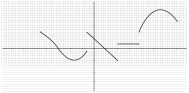
\includegraphics{../img/graficas-funciones-1.png}

\section{Gráfica 2}
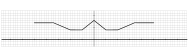
\includegraphics{../img/graficas-funciones-2.png}

\section{Gráfica 3}
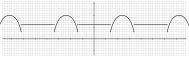
\includegraphics{../img/graficas-funciones-3.png}

\section{Gráfica 4}
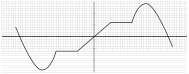
\includegraphics{../img/graficas-funciones-4.png}

\section{Gráfica 5}
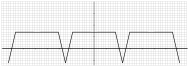
\includegraphics{../img/graficas-funciones-5.png}

\section{Gráfica 6}
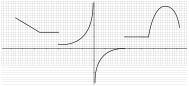
\includegraphics{../img/graficas-funciones-6.png}

\section{Gráfica 7}
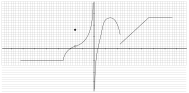
\includegraphics{../img/graficas-funciones-7.png}

\section{Gráfica 8}
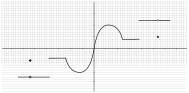
\includegraphics{../img/graficas-funciones-8.png}

\section{Gráfica 9}
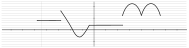
\includegraphics{../img/graficas-funciones-9.png}

\section{Gráfica 10}
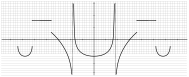
\includegraphics{../img/graficas-funciones-10.png}

\section{Gráfica 11}
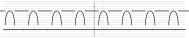
\includegraphics{../img/graficas-funciones-11.png}

\section{Gráfica 12}
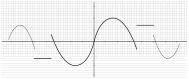
\includegraphics{../img/graficas-funciones-12.png}


\twocolumn

\end{document}
